\documentclass[
	letterpaper, % Paper size, specify a4paper (A4) or letterpaper (US letter)
	10pt, % Default font size, specify 10pt, 11pt or 12pt
]{template}

\title{Comparing energy estimators for particle detector calibration.}

\author{Sebastien Psarianos}
\newcommand{\bref}[2]{\textbf{\hyperref[#1]{#2}}}

\date{\today}

\begin{document}
\renewcommand{\lstlistingname}{Function}

\maketitle

\section{Introduction}
In this report, the accuracy of different energy estimators for calibration of a simulated particle detector was compared. The most accurate method of energy estimation was then used to analyze a set of unknown particle detection events. Particle detector calibration is a key process in high energy physics experiments and is a required step to converting raw measurement data into quantifiable energy measurements \cite{Hanagaki2022}. The simulated particle detector emits a measurable voltage signal when a particle detection event occurs. This voltage signal is a pulse that follows the form of \textbf{\hyperref[eqn-1]{Equation 1}}:
\begin{equation}
	\label{eqn-1}
	y = A \cdot(e^{-t/\tau_{\rm rise}} - e^{-t/\tau_{\rm fall}})
\end{equation}
For some amplitude $A$, $\tau_{\rm rise}= 20\unit{\micro s}$, $\tau_{\rm fall} =80\unit{\micro s}$. Every pulse begins at exactly $1000\unit{\mu s}$ due to an idealized triggering system. \cite{labManual} \textbf{\hyperref[fig::pulseSim]{Figure 1}} shows an example of a theoretical pulse with amplitude 1 (plotted with \textbf{\hyperref[lst-8]{Function 8}}). An energy estimator aims to use this voltage signal to estimate the energy of the detected particle.
\begin{figure}[H]
	\centering
	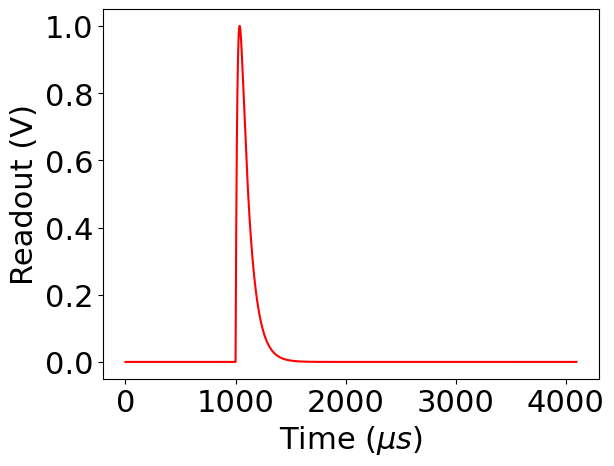
\includegraphics[width=.6\textwidth]{figures/pulses_sim.png}
	\caption{Plot of theoretical pulse model with amplitude 1~\label{fig::pulseSim}}
\end{figure}
The data that was analyzed includes two sets of 1000 samples. The first set of samples contained simulated detection events for a $10\unit{KeV}$ particle. The second set of samples contained a number of unknown detection events to be analyzed. In both cases samples consist of 4096 voltage values, each corresponding to $1\unit{\micro s}$ intervals.
\textbf{\hyperref[fig::pulseCal]{Figure 2}} and \textbf{\hyperref[fig::pulseSig]{Figure 3}} display 10 samples from the first and second data sets respectively.
\begin{figure}[H]
	\begin{minipage}[t]{0.45\textwidth}
		\centering
		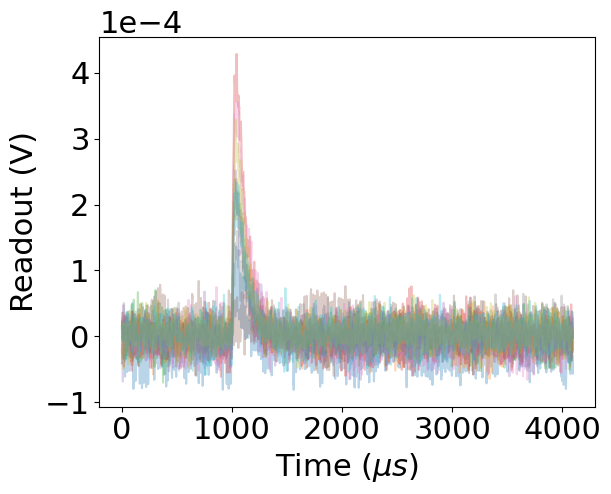
\includegraphics[width=\textwidth]{figures/pulses_cal.png}
		\caption{10 sample $10\unit{KeV}$ particle detection events from the calibration data set.~\label{fig::pulseCal}}
	\end{minipage}
	\hfill
	\begin{minipage}[t]{0.45\textwidth}
		\centering
		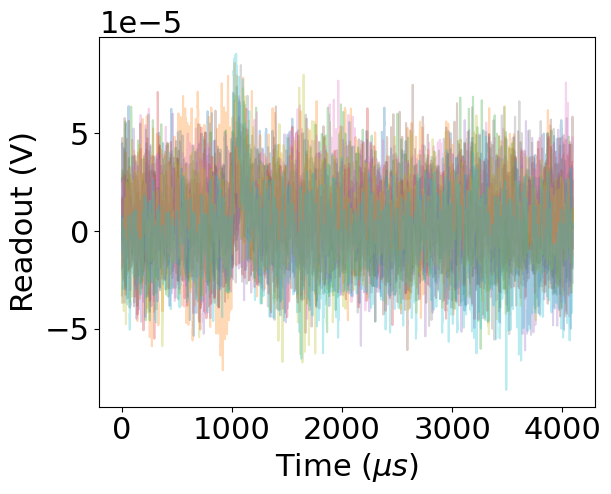
\includegraphics[width=\textwidth]{figures/pulses_signal.png}
		\caption{10 sample unknown energy pulses from the analysis data set.~\label{fig::pulseSig}}
	\end{minipage}
\end{figure}
\section{Methodology}\label{sec::method}
\subsection{Energy Estimators}
Six different energy estimation strategies were compared in this lab. They are as follows:\\
\begin{enumerate}
	\item\textbf{\hyperref[est-1]{Estimator 1}}: Maximum detected value - minimum detected value
	\item\textbf{\hyperref[est-2]{Estimator 2}}: Maximum detected value - minimum detected value - mean of 1ms pre pulse region
	\item\textbf{\hyperref[est-3]{Estimator 3}}: Approximation of integral over whole sample
	\item\textbf{\hyperref[est-4]{Estimator 4}}: Approximation of integral over whole sample - mean of 1ms pre pulse region
	\item\textbf{\hyperref[est-5]{Estimator 5}}: Approximation of area under pulse - mean of 1ms pre pulse region
	\item\textbf{\hyperref[est-6]{Estimator 6}}: Amplitude of theoretical pulse model best fit - mean of 1ms pre pulse region\\
\end{enumerate}
All of these energy estimators along with their python implementations are detailed in \textbf{\hyperref[sec::estimators]{B Energy Estimators}}.
\subsection{Calibration}\label{sec::method-calibration}
Each energy estimator was applied to each sample in the calibration data, giving a distribution of each sample's energy estimation value. These distributions were then binned into one histogram for each energy estimation method and fit to a Gaussian distribution. This was done using scipy.optimize curve\_fit and \textbf{\hyperref[lst-9]{Function 9}}.\\\\
For every energy estimator, there was visually a Gaussian shape present in the data. However, this was generally surrounded by a fairly constant bin height. This is likely due to background interference from other electrical signals or particles present in the environment. Therefore, the range of values that were binned was reduced to be inside the maximum and minimum measured values to reduce impact on the fit. This improved the $\chi^2$ probability of all the Gaussian fits. Additionally, bin numbers were adjusted manually by trial and error for each histogram to improve the same metric. \\\\
A conversion factor is required for each estimator to convert the values from $(\unit{mV})$ into $(\unit{KeV})$ to reflect the particle energy. This data set contains particle detection events in the region of the $10\unit{KeV}$ energy level. Therefore, a calibration factor was found for each estimator that, when multiplied by every value, would result in a Gaussian mean at $10\unit{KeV}$. Additionally, the $\sigma$ parameter of the Gaussian distribution was recorded as this provided an estimation of the resolution of the estimation method.\\\\
The calibration factor was applied to each voltage value. This gave new a calibrated energy distribution for each energy estimation strategy. Using the same bin ranges (converted to the new scale using the calibration factor) and bin numbers, these were then re-binned, re-fit and re-plotted using the same strategies as the non calibrated data. The pre and post-calibration graphs are displayed in \textbf{\hyperref[sec::energyEst]{Section A}} in the appendix.

\subsection{Data Analysis}
After comparing each of these methods, the best was determined to be \textbf{\hyperref[est-5]{Estimator 5}}. The analysis that lead to this decision is discussed in \textbf{\hyperref[sec::res]{Section 3}}. Once this had been determined, \textbf{\hyperref[est-5]{Estimator 5}} was applied to every sample in the analysis data set and then calibrated using its previously determined calibration value from \bref{sec::method-calibration}{Section 2.2}. This gave an estimated particle energy for each detection event in the analysis data set.\\\\
Once the data had been binned into a histogram, it seemed to have the form of exponential decay. Thus, to test this hypothesis, \textbf{\hyperref[lst-10]{Function 10}} was defined and was fit to the data using scipy.optimize curve\_fit (Displayed in \textbf{\hyperref[fig::6]{Figure 6}}).\\\\
A good fit was achieved without cutting off any of the ends of the distribution. However, there was a bin that had a small amount of entries that was in the region below zero energy. Since it does not make sense for a particle to deposit zero energy, it was removed from the data. As usual, the bin number was adjusted to get a good fit.
\section{Results and Analysis}\label{sec::res}
\subsection{Calibration}
For each of the estimator methods, \bref{fig::4} lists the energy resolution (Gaussian $\sigma$ for the post-calibration data), number of bins used in the fit, the calibration factor that was calculated and the fit's $\chi^2$ probability.
\begin{figure}[H]\label{fig::4}
\centering
\begin{center}
\begin{tabular}[pos]{|l|c|c|c|c|c|}
		\hline
		\textbf{Method}&\textbf{Energy Resolution}&\textbf{Bins}&\textbf{Calibration Factor}&\textbf{$\chi^2$ Prob}\\
		\hline
		\textbf{1}&$0.453\unit{KeV}$&$20$&$32.8\unit{ {KeV} \per{mV} }$&94.9\%\\
		\textbf{2}&$0.546\unit{KeV}$&$20$&$32.8\unit{ {KeV} \per{mV} }$&92.8\%\\
		\textbf{3}&$15.0\unit{KeV}$&$20$&$1470.0\unit{ {KeV} \per{mV} }$&94.5\%\\
		\textbf{4}&$4.56\unit{KeV}$&$30$&$1510.0\unit{ {KeV} \per{mV} }$&98.0\%\\
		\textbf{5}&$0.244\unit{KeV}$&$32$&$59.2\unit{ {KeV} \per{mV} }$&95.2\%\\
		\textbf{6}&$0.817\unit{KeV}$&$35$&$46.8\unit{ {KeV} \per{mV} }$&94.9\%\\
		\hline
\end{tabular}
\end{center}
\caption{Comparison of energy estimators}
\end{figure}
The $\chi^2$ probability was high for each of the energy estimators. Therefore, there is clearly a Gaussian form in the data. However, there is a distinct difference in the energy resolution of the different methods.\\\\
\bref{est-5}{Estimator 5} had the lowest energy resolution. This could be due to the fact that it is measuring the mean value only during the pulse and is not affected by the surrounding noise. The idealized trigger system does not produce inconsistent pulse onset or duration \cite{labManual}. Due to this, the region of the sample that contains the pulse can be accurately targeted for analysis. This further reduces the probability that any data outside the pulse will be factored into the mean value.
\begin{figure}[H]
	\centering
	\begin{minipage}[t]{0.45\linewidth}
	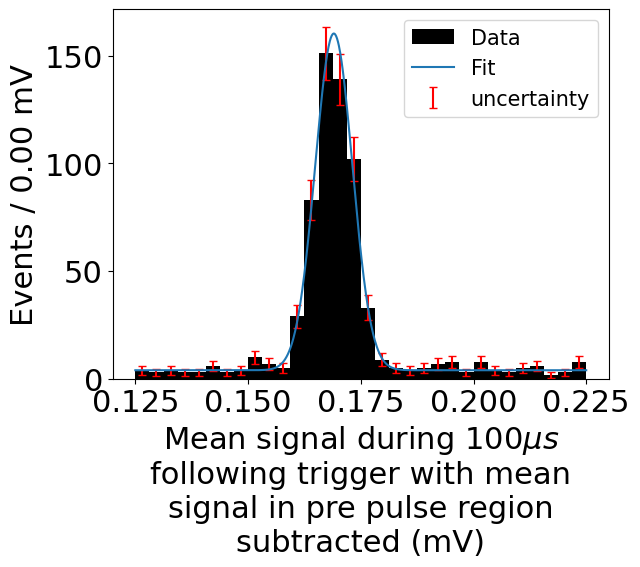
\includegraphics[width=\textwidth]{figures/area3.png}
	\caption{
		$10\unit{KeV}$ calibration particle detection events, grouped by pre-calibration energy estimate, overlaid with Gaussian best fit.\\
		\textbf{Energy Estimate}: Mean detected signal in the $100\unit{\micro s}$ after pulse start minus mean pre pulse signal  ($\unit{mV}$)
	}
	\end{minipage}
\end{figure}
\bref{est-1}{Estimator 1} and \bref{est-2}{Estimator 2} also have a relatively low energy resolution. This is possibly due to the fact that the maximum detected value that they both depend on is most likely within the pulse itself. The subtraction of the pre pulse mean value, from \bref{est-1}{Estimator 1} to \bref{est-2}{Estimator 2} actually created a worse resolution. The values are so close that more testing would be required to verify if this difference is statistically significant.\\\\
\bref{est-3}{Estimator 3} has the largest energy resolution. Since this estimation was based on every single value that was measured during the entire pulse and had no pre pulse noise removal like \bref{est-4}{Estimator 4}, this likely lead the method to be affected the most by the background interference present in the system.\\\\
\bref{est-4}{Estimator 4} had a significantly lower energy resolution than \bref{est-3}{Estimator 3}. Considering the only difference between the two estimators is the subtraction of the pre pulse mean, and since they have such differing resolutions, this strongly suggests that the pre pulse mean subtraction was beneficial for the "integral type" estimators. Both \bref{est-3}{Estimator 3} and \bref{est-4}{Estimator 4} had  high energy resolutions compared to the other methods. Considering that they take a mean over the whole sample, including the non pulse noise, this likely lead to them being the most affected by the background noise.\\\\
\bref{est-6}{Estimator 6} had a relatively low energy resolution. However, since it was not implemented with a mean pre pulse subtraction like many of the other estimators, there is a chance that this could have improved the results. Especially considering the model that was used to fit each pulse (\textbf{\hyperref[lst-7]{Function 7}}) did not have any sort of base parameter that would vertically translate it and allow it to be fit to a "base noise level". Future analysis would ideally include another estimator that added either a base parameter to the curve fit or a pre pulse mean subtraction.

\subsection{Analysis}
Considering the success of \textbf{\hyperref[est-5]{Estimator 5}} discussed in the previous section, its calibration was chosen to analyze the second data set. As discussed in \textbf{\hyperref[sec::method]{Section 2}}, this calibration data was applied to the second data set and this distribution is displayed in \textbf{\hyperref[fig::6]{Figure 6}}.
\begin{figure}[H]
\centering
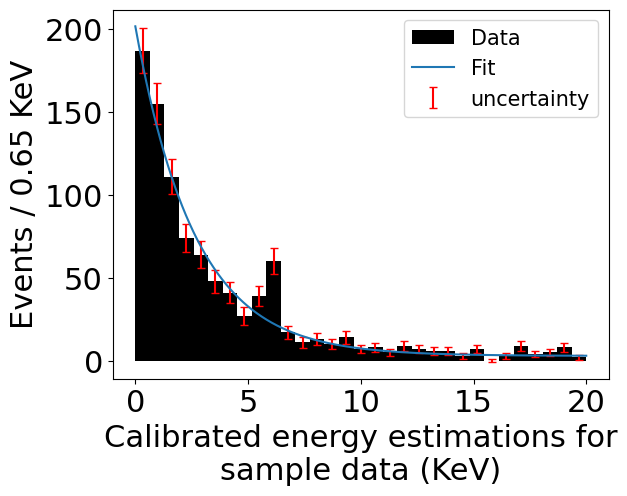
\includegraphics[width=.45\textwidth]{figures/signalAnalysis--calibrated.png}
\caption{\textbf{Energy Estimate}: Max detected signal ($\unit{mV}$).~\label{fig::6}}
\end{figure}
The $\chi_{\rm red}^2$ was approximately $2.29$. The fit was an exponential of the form $Ae^{-bx} + c$ with best fit values: $A=199, b =0.379, c = 2.87$. One noted exception to the fit was a large bin around the region of 6. This possibly could be a Gaussian or similar peak distribution of a specific energy level. Future analysis could attempt to fit this section of the distribution better. The overall trend however, seems to be of the form of exponential decay.
\section{Conclusion}
The purpose of this lab was to compare the effectiveness of various energy estimators for this simulated particle detector, using a calibration data set. Then to use this data to analyze an unknown data set. It became clear through the process of analysis that the effectiveness of an energy estimator was primarily dependent on how much it weighted regions of the sample that were outside the pulse. Future expansions to this analysis should include more investigation into refining the "integral type" methods and the pulse fit method. Additionally, more sophisticated methods for reducing the noise, such as fitting the noise data to a normal distribution would likely create a more reliable way to reduce interference. The analysis of the unknown data was relatively successful, however exploring more complex fitting functions could result in a better data fit.
\newpage\appendix{}
\section{Energy Estimator Graphs}\label{sec::energyEst}
\begin{figure}[H]
	\begin{minipage}[t]{0.45\linewidth}
		\begin{center}
            \label{fig::amp1}
			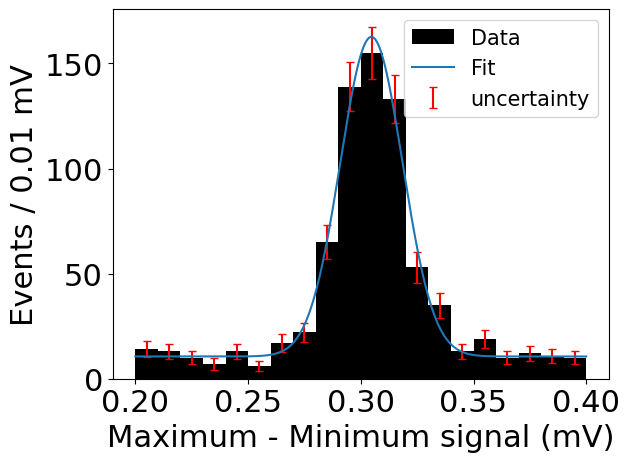
\includegraphics[width=\textwidth]{figures/amp1.png}
			\caption{
                $10\unit{KeV}$ calibration particle detection events, grouped by pre-calibration energy estimate, overlaid with Gaussian best fit.\\
                \textbf{Energy Estimate}: Max - Min detected signal ($\unit{mV}$).
            }
		\end{center}
	\end{minipage}
    \hfill
	\begin{minipage}[t]{0.45\linewidth}
		\begin{center}
            \label{fig::amp1--cal}
			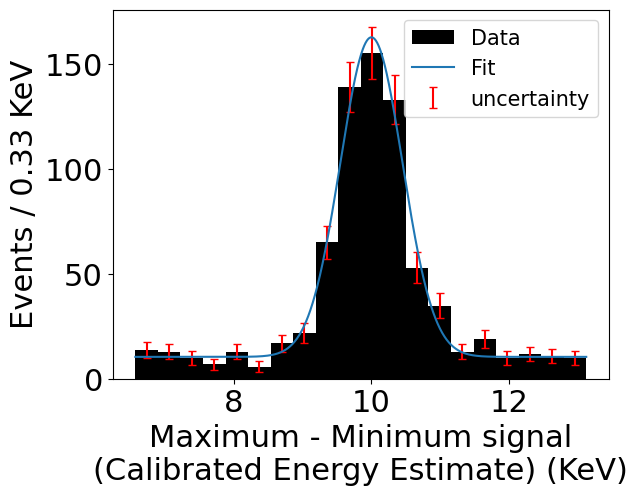
\includegraphics[width=\textwidth]{figures/amp1--calibrated.png}
			\caption{
                $10\unit{KeV}$ calibration particle detection events, grouped by calibrated energy estimate, overlaid with Gaussian best fit. x-axis has been proportionally calibrated to place Gaussian fit mean at $10\unit{KeV}$ \\
                \textbf{Energy Estimate}: Max - Min detected signal ($\unit{mV}$).
            }
		\end{center}
	\end{minipage}
\end{figure}

\begin{figure}[H]
	\begin{minipage}[t]{0.45\linewidth}
		\begin{center}
            \label{fig::amp2}
			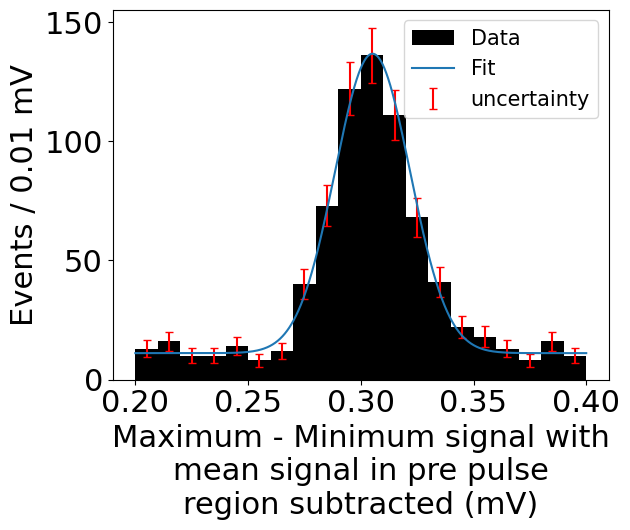
\includegraphics[width=\textwidth]{figures/amp2.png}
			\caption{
                $10\unit{KeV}$ calibration particle detection events, grouped by pre-calibration energy estimate, overlaid with Gaussian best fit.\\
                \textbf{Energy Estimate}: Max detected signal minus mean pre pulse signal  ($\unit{mV}$)
            }
		\end{center}
	\end{minipage}
    \hfill
	\begin{minipage}[t]{0.45\linewidth}
		\begin{center}
            \label{fig::amp2--cal}
			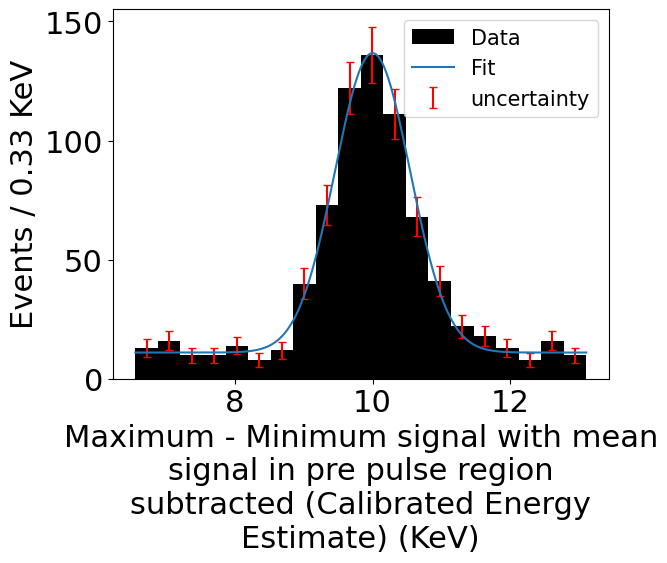
\includegraphics[width=\textwidth]{figures/amp2--calibrated.png}
			\caption{
                $10\unit{KeV}$ calibration particle detection events, grouped by calibrated energy estimate, overlaid with Gaussian best fit. x-axis has been proportionally calibrated to place Gaussian fit mean at $10\unit{KeV}$ \\
                \textbf{Energy Estimate}: Max detected signal ($\unit{mV}$) minus mean pre pulse signal
            }
		\end{center}
	\end{minipage}
\end{figure}
\begin{figure}[H]
	\begin{minipage}[t]{0.45\linewidth}
		\begin{center}
            \label{fig::area1}
			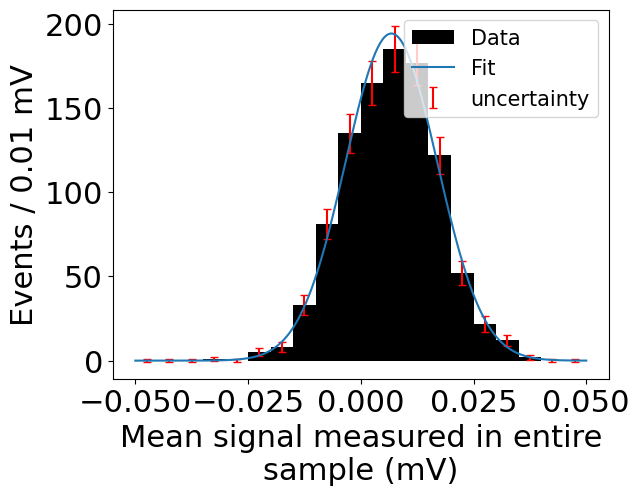
\includegraphics[width=\textwidth]{figures/area1.png}
			\caption{
                $10\unit{KeV}$ calibration particle detection events, grouped by pre-calibration energy estimate, overlaid with Gaussian best fit.\\
                \textbf{Energy Estimate}: Mean detected signal ($\unit{mV}$)
            }
		\end{center}
	\end{minipage}
    \hfill
	\begin{minipage}[t]{0.45\linewidth}
		\begin{center}
            \label{fig::area1--cal}
			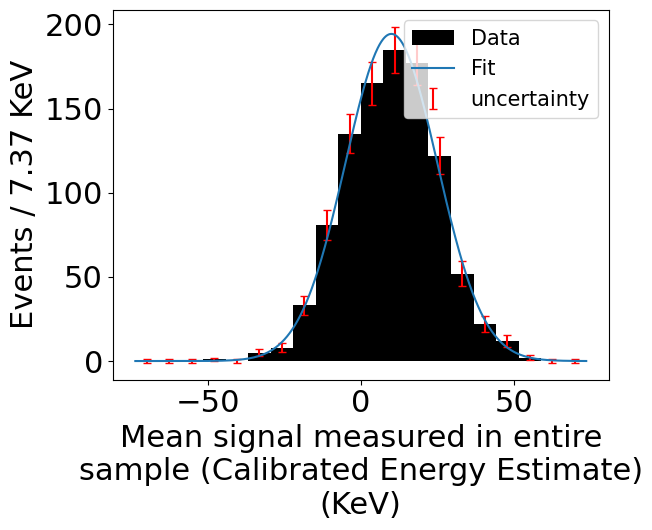
\includegraphics[width=\textwidth]{figures/area1--calibrated.png}
			\caption{
                $10\unit{KeV}$ calibration particle detection events, grouped by calibrated energy estimate, overlaid with Gaussian best fit. x-axis has been proportionally calibrated to place Gaussian fit mean at $10\unit{KeV}$ \\
                \textbf{Energy Estimate}: Mean detected signal ($\unit{mV}$)
            }
		\end{center}
	\end{minipage}
\end{figure}

\begin{figure}[H]
	\begin{minipage}[t]{0.45\linewidth}
		\begin{center}
            \label{fig::area2}
			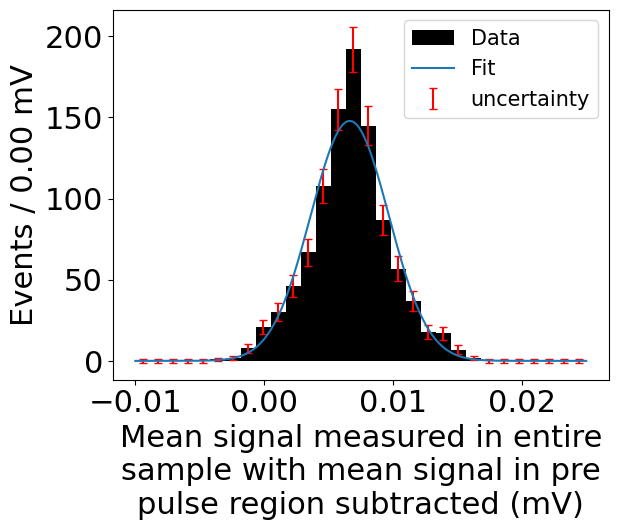
\includegraphics[width=\textwidth]{figures/area2.png}
			\caption{
                $10\unit{KeV}$ calibration particle detection events, grouped by pre-calibration energy estimate, overlaid with Gaussian best fit.\\
                \textbf{Energy Estimate}: Mean detected signal minus mean pre pulse signal  ($\unit{mV}$)
            }
		\end{center}
	\end{minipage}
    \hfill
	\begin{minipage}[t]{0.45\linewidth}
		\begin{center}
            \label{fig::area2--cal}
			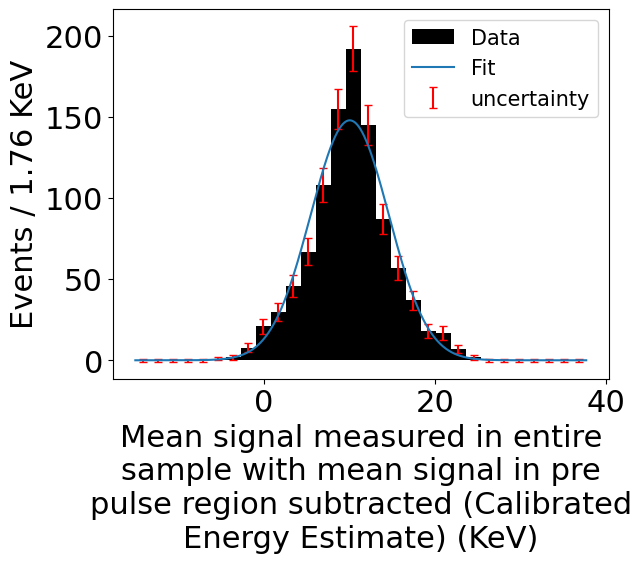
\includegraphics[width=\textwidth]{figures/area2--calibrated.png}
			\caption{
                $10\unit{KeV}$ calibration particle detection events, grouped by calibrated energy estimate, overlaid with Gaussian best fit. x-axis has been proportionally calibrated to place Gaussian fit mean at $10\unit{KeV}$ \\
                \textbf{Energy Estimate}: Mean detected signal minus mean pre pulse signal  ($\unit{mV}$)
            }
		\end{center}
	\end{minipage}
\end{figure}


\begin{figure}[H]
	\begin{minipage}[t]{0.45\linewidth}
		\begin{center}
            \label{fig::area3}
			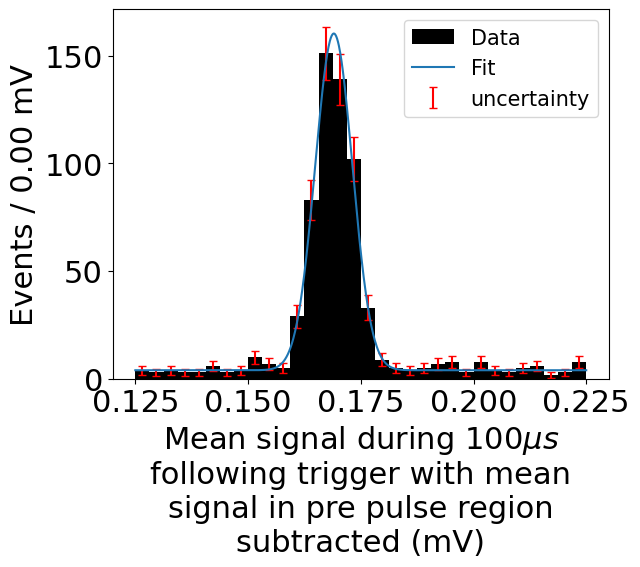
\includegraphics[width=\textwidth]{figures/area3.png}
			\caption{
                $10\unit{KeV}$ calibration particle detection events, grouped by pre-calibration energy estimate, overlaid with Gaussian best fit.\\
                \textbf{Energy Estimate}: Mean detected signal in the $100\unit{\micro s}$ after pulse start minus mean pre pulse signal  ($\unit{mV}$)
            }
		\end{center}
	\end{minipage}
    \hfill
	\begin{minipage}[t]{0.45\linewidth}
		\begin{center}
            \label{fig::area3--cal}
			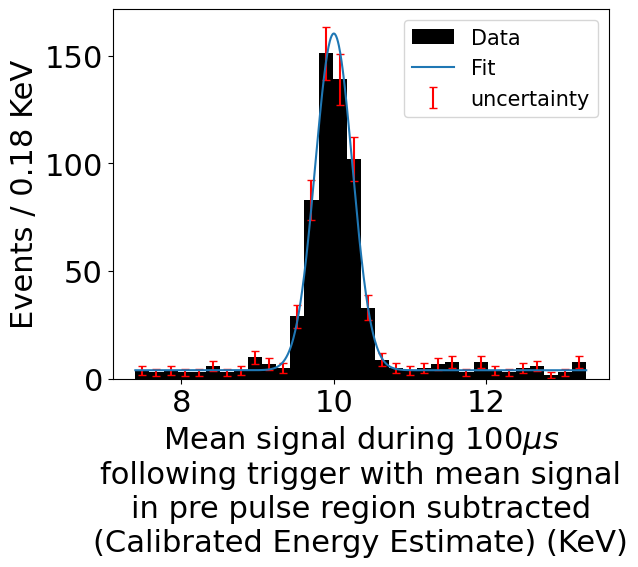
\includegraphics[width=\textwidth]{figures/area3--calibrated.png}
			\caption{
                $10\unit{KeV}$ calibration particle detection events, grouped by calibrated energy estimate, overlaid with Gaussian best fit. x-axis has been proportionally calibrated to place Gaussian fit mean at $10\unit{KeV}$ \\
                \textbf{Energy Estimate}: Mean detected signal in the $100\unit{\micro s}$ after pulse start minus mean pre pulse signal  ($\unit{mV}$)
            }
		\end{center}
	\end{minipage}
\end{figure}
\begin{figure}[H]
	\begin{minipage}[t]{0.45\linewidth}
		\begin{center}
            \label{fig::pulseFit}
			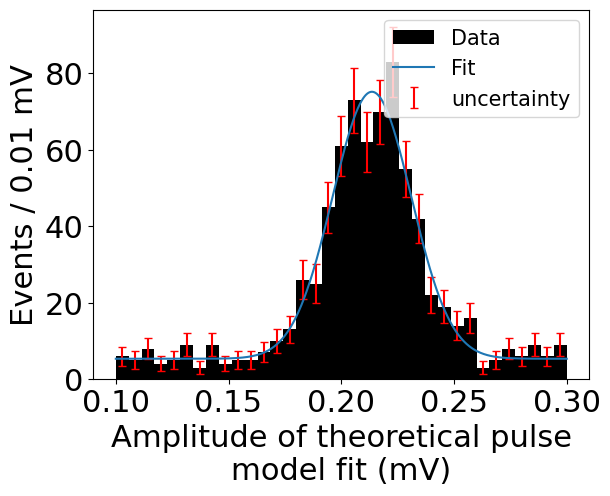
\includegraphics[width=\textwidth]{figures/pulseFit.png}
			\caption{
                $10\unit{KeV}$ calibration particle detection events, grouped by pre-calibration energy estimate, overlaid with Gaussian best fit.\\
                \textbf{Energy Estimate}: Amplitude of theoretical pulse model fit (mV)
            }
		\end{center}
	\end{minipage}
    \hfill
	\begin{minipage}[t]{0.45\linewidth}
		\begin{center}
            \label{fig::pulseFit--cal}
			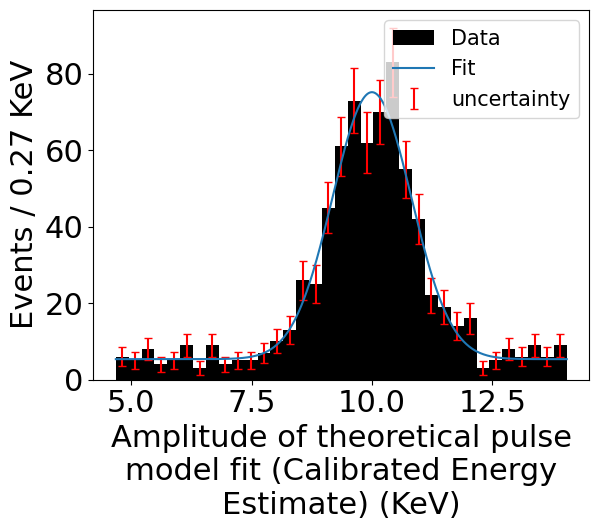
\includegraphics[width=\textwidth]{figures/pulseFit--calibrated.png}
			\caption{
                $10\unit{KeV}$ calibration particle detection events, grouped by calibrated energy estimate, overlaid with Gaussian best fit. x-axis has been proportionally calibrated to place Gaussian fit mean at $10\unit{KeV}$ \\
                \textbf{Energy Estimate}: Amplitude of theoretical pulse model fit (mV)
            }
		\end{center}
	\end{minipage}
\end{figure}

\newpage
\section{Energy Estimators}\label{sec::estimators}
For any given sample, $\{V_i \}$ is the set of voltage readings in that sample.\\\\
\begin{minipage}[t]{.45\textwidth}
{\large\textbf{Estimator 1: Amplitude Estimator 1}~\label{est-1}}\\
Implementation: \textbf{\hyperref[lst-1]{Function 1}}\\\\
This estimator takes the largest voltage value measured during the pulse and subtracts the smallest value measured during the pulse. This gives an estimation of the height of the pulse.
\[E\propto \max{V_i} - \min{V_i}\]
\end{minipage}
\hfill
\begin{minipage}[t]{.45\textwidth}
{\large\textbf{Estimator 2: Amplitude Estimator 2}~\label{est-2}}\\
Implementation: \textbf{\hyperref[lst-2]{Function 2}}\\\\
This estimator is similar to \textbf{\hyperref[est-1]{Estimator 1}}. It subtracts the minimum voltage from the maximum voltage. Additionally, however, it calculates the mean of the first 1ms pre pulse region and subtracts this to approximate the noise of the system.
\begin{align*}
E&\propto \max{V_i} - \min{V_i} - \underbrace{{1\over 1000}\sum_i^{1000} V_i }_{\text {pre pulse mean}} \\ &= \max{V_i} - \min{V_i} - \langle V_i \rangle_{i\in\{0,...,1000\}}
\end{align*}
\end{minipage}\\\\

\begin{minipage}[t]{.45\textwidth}
{\large\textbf{Estimator 3: Area Estimator 1}~\label{est-3}}\\
Implementation: \textbf{\hyperref[lst-3]{Function 3}}\\\\
The purpose of this estimator is to approximate integration over the entire sample. The integral can be approximated with a sum over all the measured values as a Riemann sum with $\Delta x = 1$:
\[ \sum_{i=1}^{4096} V_i \approx\int_0^{4096}V(t)\dd{t} \]
This is equivalent to the mean value multiplied by the number of elements. Since proportionality is all that is required, the mean value is used.
\[ E \propto \cdot \langle V_i\rangle \propto \sum_{i=1}^{4096} V_i \]\\\\
\end{minipage}
\hfill
\begin{minipage}[t]{.45\textwidth}
{\large\textbf{Estimator 4: Area Estimator 2}~\label{est-4}}\\
Implementation: \textbf{\hyperref[lst-4]{Function 4}}\\\\
This estimator is identical to \textbf{\hyperref[est-3]{Estimator 3}} but with the same the pre pulse mean subtraction from \textbf{\hyperref[est-2]{Estimator 2}}
\[ E \propto \langle V_i\rangle - \langle V_i \rangle_{i\in\{0,...,1000\}}\]
\end{minipage}\\\\
\begin{minipage}[t]{.45\textwidth}
{\large\textbf{Estimator 5: Area Estimator 3}~\label{est-5}}\\
Implementation: \textbf{\hyperref[lst-5]{Function 5}}\\\\
This estimator aims to refine \textbf{\hyperref[est-4]{Estimator 4}} by reducing the noise that is picked up outside the pulse. This is done by taking the mean value of only the section of the sample that contains the pulse. Due to the idealized trigger system, every pulse starts at 100$\mu s$ with a 20$\mu s$ rise and 80$\mu s$ decay \cite{labManual} . Therefore, the mean is taken over the interval of time from $t=100\unit{\micro s} \rightarrow 200\unit{\micro s}$
\begin{align*}
	E &\propto {1 \over 2000} \sum_{i=1000}^{1100} V_i - \langle V_i \rangle_{i\in\{0,...,1000\}}\\
	&= \langle V_i\rangle _{i\in\{1000, ... ,1100\}} - \langle V_i \rangle_{i\in\{0,...,1000\}}
\end{align*}
\end{minipage}
\hfill
\begin{minipage}[t]{.45\textwidth}
{\large \textbf{Estimator 6: Curve Fit}~\label{est-6}}\\
Implementation: \textbf{\hyperref[lst-6]{Function 6}}\\\\
This fit method used the scipy.optimize curve\_fit function in conjunction with \textbf{\hyperref[lst-7]{Function 7}} to fit each sample using the theoretical model defined in \textbf{\hyperref[eqn-1]{Equation 1}}. The best fit of the amplitude value was then returned as the energy estimation.
\end{minipage}\\\\
\newpage

\section{Functions}
\begin{lstlisting}[caption={\label{lst-1}Implementation of \textbf{\hyperref[est-1]{Estimator 1}}},captionpos=b,language=python]
def amp1Estimator(sample):
    """Implements the first amplitude estimator and converts to mV"""
    return (np.max(sample)  - np.min(sample)) * 1000
\end{lstlisting}
\begin{lstlisting}[caption={\label{lst-2}Implementation of  \textbf{\hyperref[est-2]{Estimator 2}}},captionpos=b,language=python]
def amp2Estimator(sample):
    """Implements the second amplitude estimator and converts to mV"""
    baseline = np.average(sample[:1001])
    return (np.max(sample)  - np.min(sample) - baseline) * 1000
\end{lstlisting}
\begin{lstlisting}[caption={\label{lst-3}Implementation of  \textbf{\hyperref[est-3]{Estimator 3}}},captionpos=b,language=python]
def area1Estimator(sample):
    """Implements the first integral estimator and converts to mV"""
    return (np.mean(sample)) * 1000
\end{lstlisting}
\begin{lstlisting}[caption={\label{lst-4}Implementation of  \textbf{\hyperref[est-4]{Estimator 4}}},captionpos=b,language=python]
def area2Estimator(sample):
    """Implements the second integral estimator and converts to mV"""
    baseline = np.average(sample[:1001])
    return (np.mean(sample) - baseline ) * 1000
\end{lstlisting}
\begin{lstlisting}[caption={\label{lst-5}Implementation of  \textbf{\hyperref[est-5]{Estimator 5}}},captionpos=b,language=python]
def area3Estimator(sample):
    """Implements the third integral estimator and converts to mV"""
    baseline = np.average(sample[:1001])
    return (np.mean(sample[1001:1101]) - baseline ) * 1000
\end{lstlisting}
\begin{lstlisting}[caption={\label{lst-6}Implementation of  \textbf{\hyperref[est-6]{Estimator 6}}},captionpos=b,language=python]
def pulseFitEstimator(sample):
    """Implements the pulse fit estimator and converts to mV"""
    return curve_fit(fit_pulse, np.linspace(0, 4095, 4096), sample )[0] * 1000
\end{lstlisting}
\begin{lstlisting}[caption={\label{lst-7} Function used in the fitting process for \textbf{\hyperref[est-6]{Estimator 6}} uses \textbf{\hyperref[lst-8]{Function 8}} as theoretical model}  model,captionpos=b,language=python]
def fit_pulse(x, A):
    _pulse_template = pulse_shape(20,80)
    xx=np.linspace(0, 4095, 4096)
    return A*np.interp(x, xx, _pulse_template)
\end{lstlisting}
\begin{lstlisting}[caption={\label{lst-8} Python implementation of \textbf{\hyperref[eqn-1]{Equation 1}}},
captionpos=b,language=python]
def pulse_shape(t_rise, t_fall):
    xx=np.linspace(0, 4095, 4096)
    yy = -(np.exp(-(xx-1000)/t_rise)-np.exp(-(xx-1000)/t_fall))
    yy[:1000]=0
    yy /= np.max(yy)
    return yy
\end{lstlisting}
\begin{lstlisting}[caption={\label{lst-9}Implementation of gaussian distribution used to fit the calibration data},captionpos=b,language=python]
def myGauss(x, A, mean, width, base):
    return A*np.exp(-(x-mean)**2/(2*width**2)) + base
\end{lstlisting}
\begin{lstlisting}[caption={\label{lst-10}Implementation of exponential decay used to fit the calibration data},captionpos=b,language=python]
def myExp(x, A, dec, base):
    return A * np.exp(-dec * x) + base
\end{lstlisting}

\bibliographystyle{plain}
\bibliography{references.bib}

\end{document}
